\section{\large \textcolor{blue}{Óptica geométrica}}

\begin{flushleft}
\textbf{\textcolor{blue}{\Large Quest\~ao - Entrada da Fibra Óptica — Lei de Snell}}\\
\noindent

\subsection{Quest\~ao Entrada da Fibra Óptica — Lei de Snell}

\vspace{0.5cm}

\textcolor{red}{\textbf{Solução:}}\\

\section*{Índices de Refração}

\begin{itemize}
    \item $n_1 = 1$
    \item $n_2 = 1{,}6$
    \item $n_3 = 1{,}5$
\end{itemize}

\section*{Entrada da Fibra Óptica (Raio de Luz)}

Utilizando a \textbf{Lei de Snell}, temos:

\subsection*{1. Incidência do meio $n_1$ para o meio $n_2$ (ponto 1):}
\[
n_1 \cdot \sin \theta = n_2 \cdot \sin \phi
\Rightarrow \sin \theta = 1{,}6 \cdot \sin \phi
\]

\subsection*{2. Reflexão Total Interna no ponto (2):}
\[
n_2 \cdot \sin \alpha = n_3 \cdot \sin 90^\circ
\Rightarrow 1{,}6 \cdot \sin \alpha = 1{,}5 \cdot 1 = 1{,}5
\Rightarrow \sin \alpha = \frac{1{,}5}{1{,}6}
\]

\subsection*{3. Substituindo na equação de Snell:}
\[
\sin \theta = 1{,}6 \cdot \sin \phi
\qquad
\text{e}
\qquad
\sin \alpha = \frac{1{,}5}{1{,}6} = \frac{15}{16}
\]

\subsection*{4. Cálculo de $\sin \theta$:}
\[
\sin \theta = 1{,}6 \cdot \sin \phi = \frac{15}{10} = \frac{3{,}5}{4{,}4}
\]

\section*{Identidade Trigonométrica (para reflexão total):}

Sabemos que:
\[
\phi + \alpha = 90^\circ
\Rightarrow \alpha = 90^\circ - \phi
\]

Portanto:
\[
\sin (90^\circ - \phi) = \cos \phi
\quad \Rightarrow \quad
\sin \alpha = \cos \phi
\]

Logo:
\[
\sin(90^\circ - \phi) = \sin 90^\circ \cdot \cos \phi - \cos 90^\circ \cdot \sin \phi = \cos \phi
\]

Sabemos que:

\[
\cos \phi = \frac{15}{16}
\]

Pelo fato de que:
\[
\sin^2 \phi + \cos^2 \phi = 1
\Rightarrow \sin^2 \phi = 1 - \left(\frac{15}{16}\right)^2
= \frac{256 - 225}{256} = \frac{31}{256}
\]

\[
\Rightarrow \sin \phi = \sqrt{\frac{31}{256}}
\]

Agora, usando a equação:
\[
\sin \theta = 1{,}6 \cdot \sin \phi
\Rightarrow \sin \theta = 1{,}6 \cdot \sqrt{\frac{31}{256}}
= \frac{16}{10} \cdot \sqrt{\frac{31}{256}}
= \frac{16}{10} \cdot \frac{\sqrt{31}}{16}
= \frac{\sqrt{31}}{10}
\]

Portanto, o ângulo de incidência máximo é:

\[
\boxed{
\theta = \sin^{-1} \left( \frac{\sqrt{31}}{10} \right)
}
\]

\end{flushleft}


\begin{flushleft}
\textbf{\textcolor{blue}{\Large Quest\~ao 23 - IFFAR 2023 - Associa\c{c}\~ao de Lentes Delgadas}}\\
\noindent

\subsection{Quest\~ao 23 - IFFAR 2023 - Associa\c{c}\~ao de Lentes Delgadas}

Sistemas \'opticos compostos por associa\c{c}\~ao de lentes desempenham um papel fundamental no ensino de f\'isica no campo da \'optica geom\'etrica. Eles s\~ao utilizados para produzir imagens com caracter\'isticas especiais, assim como aquelas obtidas por microsc\'opios compostos ou lunetas astron\^omicas.

Nesse contexto, considere um caso te\'orico em que duas lentes delgadas, sendo elas coaxiais, s\~ao associadas com uma dist\^ancia $d = 15\,cm$ entre elas. As lentes t\^em dist\^ancias focais $f_1 = 10\,cm$ e $f_2 = 2\,cm$.

Qual \'e a verg\^encia equivalente da associa\c{c}\~ao das lentes?

\begin{itemize}
\item[(A)] $-0{,}07\,di$
\item[(B)] $-15\,di$
\item[(C)] $0{,}02\,di$
\item[(D)] $12\,di$
\item[(E)] $60\,di$
\end{itemize}

\vspace{0.5cm}

\begin{center}
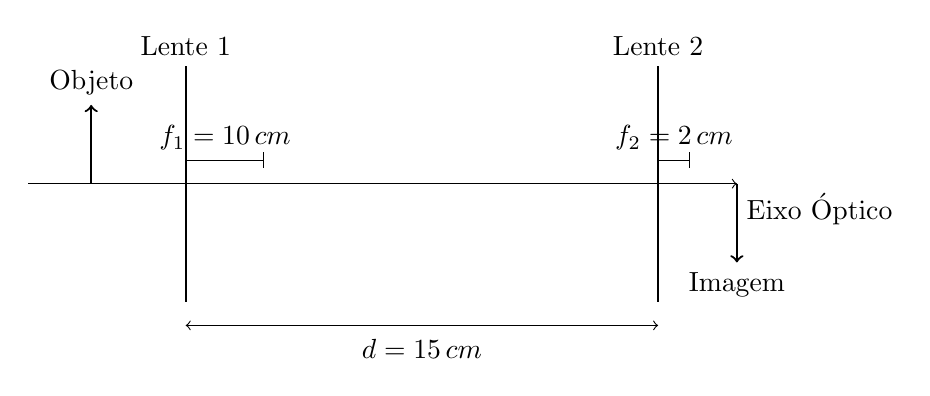
\begin{tikzpicture}[scale=1]

% Eixo principal
\draw[->] (-2,0) -- (7,0) node[below right] {Eixo Óptico};

% Lentes
\draw[thick] (0,-1.5) -- (0,1.5);
\draw[thick] (6,-1.5) -- (6,1.5);

% Rótulos das lentes
\node[above] at (0,1.5) {Lente 1};
\node[above] at (6,1.5) {Lente 2};

% Distância entre lentes
\draw[<->] (0,-1.8) -- (6,-1.8);
\node at (3,-2.1) {$d = 15\,cm$};

% Foco da lente 1 (esquerda)
\draw[|-|] (0,0.3) -- (1,0.3);
\node[above] at (0.5,0.3) {$f_1 = 10\,cm$};

% Foco da lente 2 (direita)
\draw[|-|] (6,0.3) -- (6.4,0.3);
\node[above] at (6.2,0.3) {$f_2 = 2\,cm$};

% Objeto
\draw[->, thick] (-1.2,0) -- (-1.2,1);
\node[above] at (-1.2,1) {Objeto};

% Imagem final (só referência)
\draw[->, thick] (7,0) -- (7,-1);
\node[below] at (7,-1) {Imagem};

\end{tikzpicture}
\end{center}

\textcolor{red}{\textbf{Solu\c{c}\~ao:}}\\

Quando duas lentes delgadas s\~ao associadas a uma certa dist\^ancia $d$ entre si, a verg\^encia equivalente do sistema \'optico \'{e} dada por:

\[
\boxed{
V = V_1 + V_2 - d \cdot V_1 \cdot V_2
}
\]

Onde:
\begin{itemize}
    \item $V_1 = \dfrac{100}{f_1}$, com $f_1$ em cm
    \item $V_2 = \dfrac{100}{f_2}$, com $f_2$ em cm
    \item $d$ \'e a dist\^ancia entre as lentes, em metros
\end{itemize}

Calculamos as verg\^encias individuais:

\[
V_1 = \frac{100}{10} = 10\,di
\qquad
V_2 = \frac{100}{2} = 50\,di
\]

Convertendo a dist\^ancia $d$ para metros:

\[
d = 15\,cm = 0{,}15\,m
\]

Substituindo na f\'ormula da verg\^encia equivalente:

\[
V = 10 + 50 - 0{,}15 \cdot 10 \cdot 50
\]

\[
V = 60 - 0{,}15 \cdot 500 = 60 - 75 = -15\,di
\]

\vspace{0.3cm}

Portanto, a resposta correta \'e a alternativa \colorbox{green!50}{\textbf{B)}}.

\end{flushleft}


\begin{flushleft}
\textbf{\textcolor{blue}{\Large Quest\~ao - }}\\
\noindent

\subsection{Quest\~ao }

\begin{itemize}
\item[(A)] 
\item[(B)] 
\item[(C)]
\item[(D)] 
\item[(E)] 
\end{itemize}

\vspace{0.5cm}

\textcolor{red}{\textbf{Solução:}}\\


A resposta correta é alternativa \colorbox{green!50}{\textbf{...}}.

\end{flushleft}




